
\section{mclique.rb - Enumerate Maximal Cliques\label{sect:mclique}}

This command enumerates the maximal cliques from general graph. The \verb|mace| command \cite{UnoWeb} is used in mclique.rb. 
Given $G=(V,E)$ is an undirected graph with node (referred as vertex) set $V$ and edge set $E$, 
a clique is a subset of its nodes (or vertices)  $V$ such that every two nodes in the subset are connected by an edge in the subgraph of $G$ . 
A maximal clique is a clique that is not an exclusive subset of a larger clique (Figure \ref{fig:clique}).

\begin{figure}[htbp]
\begin{center}
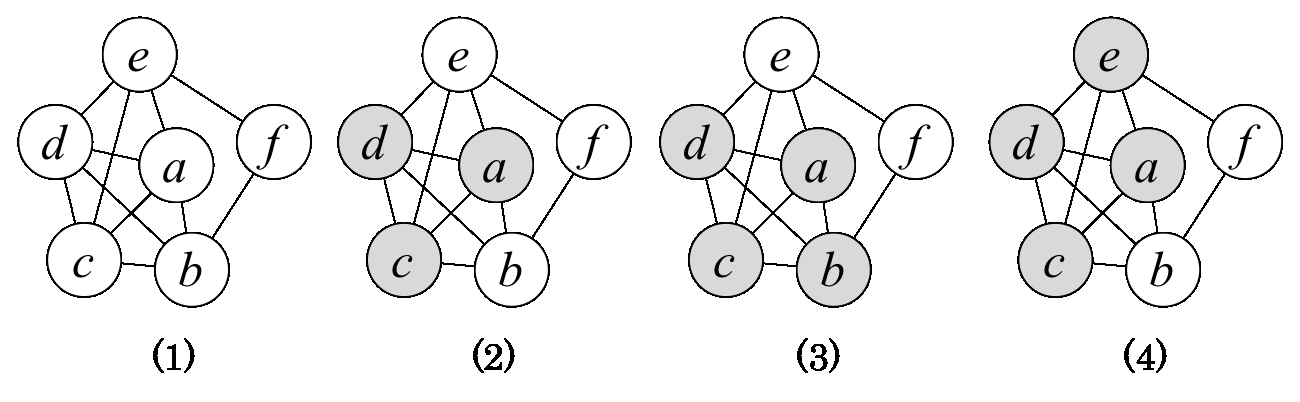
\includegraphics[scale=0.5]{./clique.eps}
\caption{General graph (1) consists of a clique in the subgraph indicated by the shaded nodes in (2),  but the subset is not maximal clique as shown in (3) and (4).  
On the other hand, (3) and (4) are maximal cliques since they are not a subset of other cliques. 
(3) and (4) is constructed by 4 nodes, with 3 common nodes. 
\label{fig:clique}}
\end{center}
\end{figure} 

In general cases, the data points grow to a huge number when enumerating maximal cliques. This is due to the fact that the nodes of maximal cliques overlap each other as shown in Figure \ref{fig:clique} (3) and (4). 
To date, there are  several proposals to overcome this problem. 
One proposal is to treat as a complete graph if the density reaches a particular level, this is known as pseudo clique. However, sometimes more pseudo cliques are enumerated then maximal cliques, and the fundamental problem is not resolved. 
Another approach is to merge similar cliques after enumerating maximal cliques, which make use of different available clustering algorithms. Although this approach is rather promising, the run time required could be a problem depending on the number of maximal cliques enumerated. The third approach is to polish the general graph before enumeration (this cleaning technique is referred to as "data polishing") to reduce the number of maximal cliques enumerated.  
Data polishing is recently proposed by Professor Uno \cite{Uno2014}, if the statistical proof of data polishing becomes more apparent, clique enumeration will become an effective methodology. 
In section  \ref{sect:mpolishing}, this technique is implemented in \verb|mpolishing.rb| command. When mpolishing is used in conjunction with this command, the number of maximal cliques  enumerated can be reduced drastically without altering the nature of the graph. 

Table \ref{tbl:cl_input} shows the input data for this command, edge data is represented in node pair in CSV format (corresponds to Figure \ref{fig:clique} (1)). 
The graph is treated as undirected graph and may have more than one island.  

Given the graph data, maximal cliques are enumerated as shown in Table \ref{tbl:cl_output}. 

The field \verb|id| denotes clique ID, this field identifies records in the same cliques. 
Clique where \verb|id|=2 corresponds to Figure \ref{fig:clique}(4), 
and clique where \verb|id|=3 corresponds to Figure \ref{fig:clique}(3). 
In addition, maximal cliques comprised of the nodes $\{e,f\}$ and $\{b,f\}$ are enumerated. 
The last column \verb|size| contains the number of nodes that made up the maximal cliques. 

%In addition, when parameters \verb|no=,ne=| are specified, the maximal clique of nodes in graph for the clique enumerated can be saved in output.  (node is referred to as clique node, and graph is referred clique node graph). 

%If there is at least 1 common nodes for 2 cliques, an edge is added between the cliques. 
 
% Table \ref{tbl:cl_output} shows the maximal clique based on the clique node graph in Figure \ref{fig:cl_clnodeg}, the output CSV data is shown in Table \ref{tbl:cl_node},\ref{tbl:cl_edge}.

\vspace{1em}

\begin{table}[htbp]
\begin{center}
\begin{tabular}{cc}

\begin{minipage}{0.5\hsize}
\begin{center}
\caption{Input Data (Edge data)\label{tbl:cl_input}}
{\small
\begin{tabular}{cc}
\hline
node1&node2 \\
\hline
a&b \\
a&c \\
a&d \\
a&e \\
b&c \\
b&d \\
b&f \\
c&d \\
c&e \\
d&e \\
e&f \\
\hline
\end{tabular} 
}
\end{center}
\end{minipage}

\begin{minipage}{0.5\hsize}
\begin{center}
\caption{Output Results\label{tbl:cl_output}}
{\small
\begin{tabular}{cccc}
\hline
id&node1&node2&size\\
\hline
0&e&f&2\\
1&b&f&2\\
2&a&c&4\\
2&a&d&4\\
2&a&e&4\\
2&c&d&4\\
2&c&e&4\\
2&d&e&4\\
3&a&b&4\\
3&a&c&4\\
3&a&d&4\\
3&b&c&4\\
3&b&d&4\\
3&c&d&4\\
\hline
\end{tabular} 
}
\end{center}
\end{minipage}

\end{tabular} 
\end{center}
\end{table} 

%\begin{figure}[htbp]
%\begin{center}
%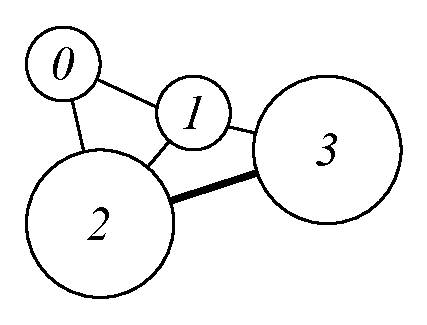
\includegraphics[scale=0.5]{./clnodeg.eps}
%\caption{Clique node graph. Table \ref{tbl:cl_output} shows 4 maximal cliques and its respective nodes for the graph. 
%The number inside the node represents an ID, the saize of the nodes are drawn in proportion to the number of nodes constituting the clique. 
%For example, clique node "2", is made up of 4 nodes $a,c,d,e$, while clique node "0" is made up of 2 nodes $e,f$. 
%When there are more than 1 common nodes between clique, an edge is extended, the thickness of the edge is drawn in proportion to the ratio. 
%For example, there is 1 common node $e$ between clique node "2" and "0".
%There is no edge between clique node "0" and "3" since there is no common node. 
%\label{fig:cl_clnodeg}}
%\end{center}
%\end{figure} 


%\begin{table}[htbp]
%\begin{center}
%\begin{tabular}{cc}

%\begin{minipage}{0.5\hsize}
%\begin{center}
%\caption{Clique node graph in node data\label{tbl:cl_node}}
%{\small
%\begin{tabular}{cc}
%\hline
%node&size \\
%\hline
%0&2 \\
%1&2 \\
%2&4 \\
%3&4 \\
%\hline
%\end{tabular} 
%}
%\end{center}
%\end{minipage}

%\begin{minipage}{0.5\hsize}
%\begin{center}
%\caption{Clique node graph in edge data\label{tbl:cl_edge}}
%{\small
%\begin{tabular}{ccc}
%\hline
%node1&node2&common \\
%\hline
%0&1&1 \\
%0&2&1 \\
%1&3&1 \\
%2&3&3 \\
%\hline
%\end{tabular} 
%}
%\end{center}
%\end{minipage}

%\end{tabular} 
%\end{center}
%\end{table} 



\subsection{Format}
\begin{verbatim}
Format) mclique.rb i= f= [o=] [l=] [u=] [-all] [-node] [-all] [-int] [log=] [T=] [--help] 

  Specify File Name 
  i=     : Edge data file 
  f=     : Column name of 2 nodes in edge data (invalid parameter when -int is specified)
  o=     : Output file (Clique ID-Edge: cliqueID-node can be modified when -node is specified)
  l=     :  Minimal number of nodes constructing the clique (clique smaller than the value 
  specified will not be enumerated) 
 u=     : Maximal number of nodes constructing the clique (clique larger than the value 
 specified will not be enumerated)
  -node  : Output in clique ID-node name pair format 
  -all   : Enumerate all cliques instead of only maximal cliques
  -int   : Process items as integers
  log=   : File name of the parameter settings saved in key based CSV format

 Others
  T= : Working directory (default:/tmp)
  --help : Help information 
\end{verbatim}

\subsection{Examples}
\subsubsection*{Example 1: Basic Example}

Example illustrated from the above section.


\begin{Verbatim}[baselinestretch=0.7,frame=single]
$ more dat1.csv
node1,node2
a,b
a,c
a,d
a,e
b,c
b,d
b,f
c,d
c,e
d,e
e,f
$ mclique.rb i=dat1.csv f=node1,node2 o=result1.csv log=log1.csv
/Users/stephane/.rvm/gems/ruby-1.9.3-p448/gems/nysol-1.5-x86_64-darwin/lib/nysol/margs.rb:
154:in `block in initialize': I don't know such a argument: `i=' (RuntimeError)
	from /Users/stephane/.rvm/gems/ruby-1.9.3-p448/gems/nysol-1.5-x86_64-darwin/lib/nysol/mar
gs.rb:152:in `each'
	from /Users/stephane/.rvm/gems/ruby-1.9.3-p448/gems/nysol-1.5-x86_64-darwin/lib/nysol/mar
gs.rb:152:in `initialize'
	from /Users/stephane/.rvm/gems/ruby-1.9.3-p448/gems/nysol-1.5-x86_64-darwin/bin/mclique.r
b:124:in `new'
	from /Users/stephane/.rvm/gems/ruby-1.9.3-p448/gems/nysol-1.5-x86_64-darwin/bin/mclique.r
b:124:in `<top (required)>'
	from /Users/stephane/.rvm/rubies/ruby-1.9.3-p448/bin/mclique.rb:23:in `load'
	from /Users/stephane/.rvm/rubies/ruby-1.9.3-p448/bin/mclique.rb:23:in `<main>'
$ more result1.csv
result1.csv: No such file or directory
$ more cn1.csv
cn1.csv: No such file or directory
$ more ce1.csv
ce1.csv: No such file or directory
$ more log1.csv
log1.csv: No such file or directory
\end{Verbatim}
\subsubsection*{Example 2: Enumerate maximal cliques with size 4 or above}



\begin{Verbatim}[baselinestretch=0.7,frame=single]
$ mclique.rb i=dat1.csv f=node1,node2 l=4 o=result2.csv
/Users/stephane/.rvm/gems/ruby-1.9.3-p448/gems/nysol-1.5-x86_64-darwin/lib/nysol/margs.rb:
154:in `block in initialize': I don't know such a argument: `i=' (RuntimeError)
	from /Users/stephane/.rvm/gems/ruby-1.9.3-p448/gems/nysol-1.5-x86_64-darwin/lib/nysol/mar
gs.rb:152:in `each'
	from /Users/stephane/.rvm/gems/ruby-1.9.3-p448/gems/nysol-1.5-x86_64-darwin/lib/nysol/mar
gs.rb:152:in `initialize'
	from /Users/stephane/.rvm/gems/ruby-1.9.3-p448/gems/nysol-1.5-x86_64-darwin/bin/mclique.r
b:124:in `new'
	from /Users/stephane/.rvm/gems/ruby-1.9.3-p448/gems/nysol-1.5-x86_64-darwin/bin/mclique.r
b:124:in `<top (required)>'
	from /Users/stephane/.rvm/rubies/ruby-1.9.3-p448/bin/mclique.rb:23:in `load'
	from /Users/stephane/.rvm/rubies/ruby-1.9.3-p448/bin/mclique.rb:23:in `<main>'
$ more result2.csv
result2.csv: No such file or directory
\end{Verbatim}
\subsubsection*{Example 3: Enumerate all cliques with size of 3}



\begin{Verbatim}[baselinestretch=0.7,frame=single]
$ mclique.rb i=dat1.csv f=node1,node2 l=3 u=3 -all o=result3.csv
/Users/stephane/.rvm/gems/ruby-1.9.3-p448/gems/nysol-1.5-x86_64-darwin/lib/nysol/margs.rb:
154:in `block in initialize': I don't know such a argument: `i=' (RuntimeError)
	from /Users/stephane/.rvm/gems/ruby-1.9.3-p448/gems/nysol-1.5-x86_64-darwin/lib/nysol/mar
gs.rb:152:in `each'
	from /Users/stephane/.rvm/gems/ruby-1.9.3-p448/gems/nysol-1.5-x86_64-darwin/lib/nysol/mar
gs.rb:152:in `initialize'
	from /Users/stephane/.rvm/gems/ruby-1.9.3-p448/gems/nysol-1.5-x86_64-darwin/bin/mclique.r
b:124:in `new'
	from /Users/stephane/.rvm/gems/ruby-1.9.3-p448/gems/nysol-1.5-x86_64-darwin/bin/mclique.r
b:124:in `<top (required)>'
	from /Users/stephane/.rvm/rubies/ruby-1.9.3-p448/bin/mclique.rb:23:in `load'
	from /Users/stephane/.rvm/rubies/ruby-1.9.3-p448/bin/mclique.rb:23:in `<main>'
$ more result3.csv
result3.csv: No such file or directory
\end{Verbatim}



